\documentclass[12pt,a4paper]{report}

% =================================================================================
% PACKAGE IMPORTS
% =================================================================================
\usepackage[utf8]{inputenc}
\usepackage[T1]{fontenc}
\usepackage{geometry}           % Page margins
\usepackage{xcolor}             % Colors
\usepackage{graphicx}           % Images
\usepackage{titlesec}           % Custom headers
\usepackage{fancyhdr}           % Footers/Headers
\usepackage{tcolorbox}          % Colored boxes
\usepackage{booktabs}           % Professional tables
\usepackage{enumitem}           % List formatting
\usepackage{hyperref}           % Hyperlinks
\usepackage{float}              % Figure placement
\usepackage{caption}            % Caption styling
\usepackage{array}              % Table column styling
\usepackage[scaled]{helvet}     % Sans-serif font
\usepackage{tikz}               % For drawing diagrams natively
\usepackage{listings}           % For code snippets
\usepackage{tabularx}           % For responsive tables
\usepackage{colortbl}           % For colored table rows
\usetikzlibrary{shapes.geometric, arrows, positioning, calc, shadows}

% =================================================================================
% CONFIGURATION & STYLING
% =================================================================================

% 1. Page Layout
\geometry{
    top=2.5cm,
    bottom=2.5cm,
    left=2.5cm,
    right=2.5cm
}

% 2. Color Palette
\definecolor{govBlue}{RGB}{0, 51, 102}      % Deep Navy
\definecolor{accentGold}{RGB}{218, 165, 32} % Gold
\definecolor{lightGray}{RGB}{245, 245, 245} % Background
\definecolor{codeGray}{RGB}{240, 240, 240}  % Code background

% 3. Typography
\renewcommand{\familydefault}{\rmdefault} % Serif for body text
\titleformat{\chapter}[display]
  {\normalfont\sffamily\huge\bfseries\color{govBlue}}
  {\chaptertitlename\ \thechapter}{20pt}{\Huge}
\titleformat{\section}
  {\normalfont\sffamily\Large\bfseries\color{govBlue}}
  {\thesection}{1em}{}
\titleformat{\subsection}
  {\normalfont\sffamily\large\bfseries\color{govBlue}}
  {\thesubsection}{1em}{}

% 4. Code Listing Style
\lstset{
    basicstyle=\ttfamily\scriptsize,
    backgroundcolor=\color{codeGray},
    frame=single,
    rulecolor=\color{gray},
    keywordstyle=\color{blue},
    commentstyle=\color{teal},
    stringstyle=\color{red},
    breaklines=true,
    showstringspaces=false,
    numbers=left,
    numberstyle=\tiny\color{gray}
}

% 5. Custom Boxes
\newtcolorbox{insightbox}[1]{
    colback=blue!5!white,
    colframe=govBlue,
    fonttitle=\bfseries\sffamily,
    title=#1,
    arc=0mm,
    boxrule=1pt
}

\newtcolorbox{techbox}[1]{
    colback=lightGray,
    colframe=gray,
    fonttitle=\bfseries\sffamily,
    title=#1,
    arc=2mm,
    boxrule=0.5pt
}

% =================================================================================
% METADATA
% =================================================================================
\hypersetup{
    colorlinks=true,
    linkcolor=govBlue,
    filecolor=magenta,      
    urlcolor=cyan,
    pdftitle={APORIS - Hackathon Report},
    pdfauthor={Team APORIS}
}

\begin{document}

% =================================================================================
% TITLE PAGE
% =================================================================================
\begin{titlepage}
    \begin{center}
        \vspace*{0.5cm}
        
        % HEADER SECTION
        {\sffamily\LARGE\bfseries\color{govBlue} UIDAI DATA HACKATHON 2026} \\[0.5cm]
        {\large National Informatics Centre (NIC) \\ Ministry of Electronics and Information Technology (MeitY)}
        
        \vspace{2.5cm}
        
        % TITLE SECTION WITH GOLD ACCENTS
        {\color{accentGold}\rule{\linewidth}{2pt}} \\[0.6cm] % Top gold line
        
        {\sffamily\Huge\bfseries\color{govBlue} APORIS} \\[0.4cm]
        {\Large\bfseries Aadhaar Predictive Operations \& Risk Intelligence System} \\[0.6cm]
        
        {\color{accentGold}\rule{\linewidth}{2pt}} % Bottom gold line
        
        \vspace{2cm}
        
        % METADATA BOX
        \begin{tcolorbox}[colback=lightGray, colframe=govBlue, width=0.95\linewidth, arc=2mm, boxrule=1.5pt]
            \centering
            \renewcommand{\arraystretch}{1.5}
            \begin{tabularx}{\linewidth}{r X}
                \textbf{\color{govBlue}Problem Statement:} & \textbf{Unlocking Societal Trends in Aadhaar Enrolment and Updates} \\
                                                           & \small \textit{Analyze patterns, anomalies, and predictive indicators to derive actionable insights for informed decision-making and system optimization.} \\
                \textbf{\color{govBlue}Theme:}             & Smart Governance / Fraud Detection \\
                \textbf{\color{govBlue}Team ID:}           & \texttt{UIDAI\_13496} \\
                \textbf{\color{govBlue}Submission Date:}   & January 20, 2026 \\
                \textbf{\color{govBlue}GitHub Repo:}       & \url{https://github.com/xxsagnikxx/aporis} \\
            \end{tabularx}
        \end{tcolorbox}
        
        \vfill
        
        % FOOTER
        \textit{Submitted by:}\\
        \textbf{Mithi Dey} (Team Lead) \\
        
        \vspace{1.5cm}
    \end{center}
\end{titlepage}

% =================================================================================
% EXECUTIVE SUMMARY
% =================================================================================
\chapter*{Executive Summary}
\addcontentsline{toc}{chapter}{Executive Summary}

The Aadhaar ecosystem generates massive volumes of enrolment and update data daily. Effective analysis of this data is critical for identifying operational risks and ensuring service quality.

\textbf{APORIS (Aadhaar Predictive Operations and Risk Intelligence System)} is an end-to-end analytics pipeline designed to transform raw API data into actionable insights. By leveraging \textbf{Time-Series Forecasting (Facebook Prophet)} and \textbf{Unsupervised Anomaly Detection (Isolation Forest)}, APORIS provides a comprehensive view of the enrolment ecosystem.

\begin{insightbox}{Key Innovations}
    \begin{itemize}
        \item \textbf{Single Source of Truth:} Aggregates Enrolment, Demographic, and Biometric data into a unified feature set.
        \item \textbf{Predictive Intelligence:} Forecasts future operational load to prevent bottlenecks.
        \item \textbf{Automated Risk Scoring:} Assigns a 0-100 risk score to every state for targeted auditing.
    \end{itemize}
\end{insightbox}

% =================================================================================
% TABLE OF CONTENTS
% =================================================================================
\tableofcontents
\newpage

% =================================================================================
% CHAPTER 1: PROBLEM STATEMENT
% =================================================================================
\chapter{Problem Statement \& Approach}

\section{The Challenge}
The government faces significant challenges in monitoring the vast network of Aadhaar enrolment centers. Manual auditing is resource-intensive and often reactive rather than proactive. 

\begin{itemize}
    \item \textbf{Data Silos:} Enrolment, demographic, and biometric data often exist in separate streams, making holistic analysis difficult.
    \item \textbf{Operational Blindspots:} Sudden spikes in updates (e.g., biometric re-captures) may indicate fraud or operator error, but are hard to detect in real-time.
    \item \textbf{Resource Allocation:} Without forecasts, it is difficult to deploy kits and operators to areas of high upcoming demand.
\end{itemize}

\section{Analytical Approach}
We adopted a multi-layered approach involving:
\begin{enumerate}
    \item \textbf{Ingestion:} Unifying disparate CSV logs.
    \item \textbf{Forecasting:} Using probabilistic models to establish baselines.
    \item \textbf{Anomaly Detection:} Using unsupervised learning to flag deviations.
    \item \textbf{Scoring:} Synthesizing metrics into a decision-support score.
\end{enumerate}

% =================================================================================
% CHAPTER 2: DATASETS USED
% =================================================================================
\chapter{Datasets Used}

\section{Data Source}
This analysis utilizes the official anonymized datasets provided by UIDAI. The data covers enrolment and update activities from \textbf{March 2, 2025, to December 31, 2025}.

\section{Dataset Description}
We consolidated the following three API datasets into a unified analytical framework:

\begin{table}[H]
    \centering
    \renewcommand{\arraystretch}{1.5}
    % FIX: Added >{\raggedright\arraybackslash} to prevent big gaps in text
    \begin{tabular}{|p{0.25\textwidth}|>{\raggedright\arraybackslash}p{0.7\textwidth}|}
        \hline
        \rowcolor{govBlue!10} \textbf{Dataset} & \textbf{Key Columns Used} \\
        \hline
        \textbf{Enrolment} & \texttt{date}, \texttt{state}, \texttt{district}, \texttt{age\_0\_5}, \texttt{age\_5\_17}, \texttt{age\_18\_+} \\
        \hline
        \textbf{Demographic Updates} & \texttt{date}, \texttt{state}, \texttt{district}, \texttt{mobile\_updates}, \texttt{address\_updates} \\
        \hline
        \textbf{Biometric Updates} & \texttt{date}, \texttt{state}, \texttt{district}, \texttt{fingerprint\_updates}, \texttt{iris\_updates} \\
        \hline
    \end{tabular}
    \caption{Description of UIDAI Datasets Used}
\end{table}

% =================================================================================
% CHAPTER 3: METHODOLOGY
% =================================================================================
\chapter{Methodology}

\section{System Architecture}

\begin{figure}[H]
    \centering
    % Resizebox ensures the diagram fits perfectly within the page margins
    \resizebox{1.0\textwidth}{!}{%
        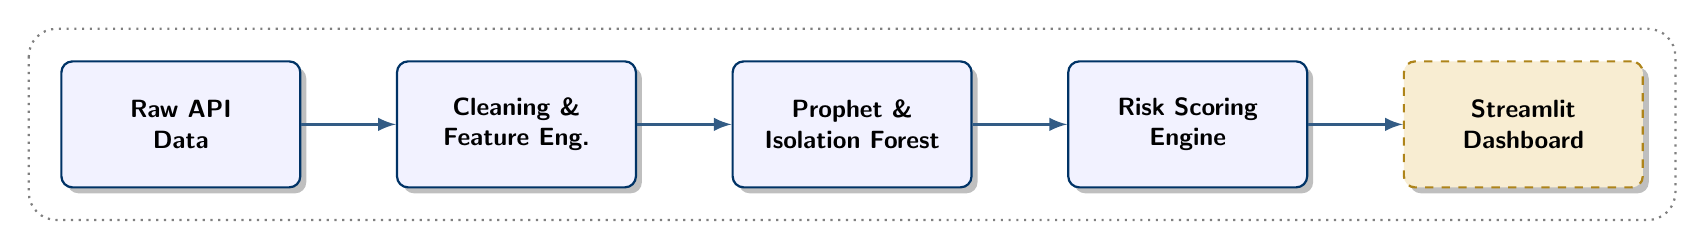
\begin{tikzpicture}[
            node distance=1.2cm,
            auto,
            >=latex', % Nice arrow tips
            % Define Professional Block Styles
            block/.style={
                rectangle,
                draw=govBlue,
                thick,
                fill=blue!5,
                text width=2.8cm,
                minimum height=1.6cm,
                text centered,
                rounded corners=4pt,
                font=\sffamily\small\bfseries,
                drop shadow % Adds 3D depth
            },
            highlight/.style={
                block,
                draw=accentGold!80!black,
                fill=accentGold!20,
                dashed
            },
            line/.style={
                draw,
                -latex,
                very thick,
                color=govBlue!80
            }
        ]

        % --- Nodes ---
        \node [block] (raw) {Raw API\\Data};
        \node [block, right=of raw] (prep) {Cleaning \&\\Feature Eng.};
        \node [block, right=of prep] (ml) {Prophet \&\\Isolation Forest};
        \node [block, right=of ml] (risk) {Risk Scoring\\Engine};
        \node [highlight, right=of risk] (dash) {Streamlit\\Dashboard};

        % --- Edges ---
        \path [line] (raw) -- (prep);
        \path [line] (prep) -- (ml);
        \path [line] (ml) -- (risk);
        \path [line] (risk) -- (dash);

        % --- Decorative Container Box ---
        \draw[dotted, thick, color=gray, rounded corners=10pt] 
            ($(raw.north west)+(-0.4,0.4)$) rectangle ($(dash.south east)+(0.4,-0.4)$);
        
        \end{tikzpicture}
    }
    \caption{APORIS End-to-End Data Pipeline Architecture}
    \label{fig:pipeline}
\end{figure}

\section{Implementation Details}

\subsection{Forecasting Engine (Module 4)}
We utilize \textbf{Facebook Prophet} to predict future operational load. The model is configured with:
\begin{itemize}
    \item \texttt{yearly\_seasonality=True}: To capture annual trends.
    \item \texttt{weekly\_seasonality=True}: To capture administrative work-week patterns.
\end{itemize}

\subsection{Anomaly Detection (Module 5)}
We employ an unsupervised \textbf{Isolation Forest} algorithm. 
\begin{itemize}
    \item \textbf{Input Features:} Standardized vectors of \texttt{update\_ratio}, \texttt{inverse\_quality}, and \texttt{future\_load\_pressure}.
    \item \textbf{Configuration:} \texttt{contamination=0.1}, \texttt{n\_estimators=100}.
\end{itemize}

\subsection{Risk Scoring Logic (Module 7)}
The final decision engine calculates a deterministic score (0-100):
\[
\text{Risk} = (10 \times \text{Update Ratio}) + (30 \times \text{Anomaly}) + (0.5 \times (100 - \text{Quality})) + \text{Cause Weight}
\]

% =================================================================================
% CHAPTER 4: DATA ANALYSIS & INSIGHTS
% =================================================================================
\chapter{Data Analysis \& Visualisation}

\section{Demographic Trends}
\begin{insightbox}{Child Enrolment Linkage}
Analysis reveals that approx. \textbf{51\% of total enrolments} correspond to children (ages 0-17), indicating strong integration between Aadhaar and birth registration/schooling systems.
\end{insightbox}

\section{Regional Anomalies}
Certain regions exhibit update behaviors that deviate significantly from the national average:
\begin{itemize}
    \item \textbf{Chandigarh:} Recorded \textbf{30,602 demographic updates} per 1,000 enrolments, reflecting high urban mobility.
    \item \textbf{Daman \& Diu:} Showed exceptional biometric update rates (\textbf{99,318 per 1,000 enrolments}), flagging potential data aggregation artifacts.
\end{itemize}

% =================================================================================
% CHAPTER 5: CONCLUSION
% =================================================================================
\chapter{Impact \& Conclusion}

\section{Impact Assessment}
\begin{itemize}
    \item \textbf{Operational Efficiency:} Reduces manual audit workload by highlighting only the top 5\% risky districts.
    \item \textbf{Fraud Prevention:} Detects non-biometric update spikes which may indicate illegal profile modifications.
    \item \textbf{Resource Optimization:} Forecasts allow better distribution of enrolment kits to high-growth zones.
\end{itemize}

\section{Conclusion}
APORIS demonstrates the power of data-driven governance. By integrating robust analytics with machine learning, it transforms raw administrative logs into a strategic asset, ensuring the integrity and efficiency of the world's largest biometric ID system.

% =================================================================================
% APPENDIX: SOURCE CODE
% =================================================================================
\appendix
\chapter{Source Code \& Notebooks}
\textit{In compliance with submission guidelines, the core analytical code used for this analysis is included below.}

\section{Module 4: Forecasting Engine (Prophet)}
\begin{lstlisting}[language=Python, caption=enrolment\_forecast.py]
import pandas as pd
from prophet import Prophet

def forecast_enrolments(days=30):
    # Load and prepare data
    df = pd.read_csv("daily_time_series.csv")
    prophet_df = df[["date", "total_enrolments"]].rename(
        columns={"date": "ds", "total_enrolments": "y"}
    )

    # Configure Model with Administrative Seasonality
    model = Prophet(
        yearly_seasonality=True,
        weekly_seasonality=True, # Captures weekend dips
        daily_seasonality=False
    )
    
    model.fit(prophet_df)
    
    # Generate Forecast
    future = model.make_future_dataframe(periods=days)
    forecast = model.predict(future)
    
    return forecast[["ds", "yhat", "yhat_lower", "yhat_upper"]]
\end{lstlisting}

\section{Module 5: Anomaly Detection (Isolation Forest)}
\begin{lstlisting}[language=Python, caption=detect\_anomalies.py]
from sklearn.ensemble import IsolationForest
from sklearn.preprocessing import StandardScaler

def detect_operational_anomalies(df):
    features = df[[
        "update_ratio", 
        "inverse_quality_score", 
        "future_load_pressure"
    ]]
    
    # Scaling is crucial for distance-based outliers
    scaler = StandardScaler()
    scaled_features = scaler.fit_transform(features)
    
    # Isolation Forest
    model = IsolationForest(
        n_estimators=100, 
        contamination=0.1, 
        random_state=42
    )
    
    df["anomaly_flag"] = model.fit_predict(scaled_features)
    return df
\end{lstlisting}

\section{Module 7: Risk Scoring Engine}
\begin{lstlisting}[language=Python, caption=risk\_score\_engine.py]
def calculate_risk(row):
    # Weighted Risk Formula
    update_risk = row["update_ratio"] * 10
    quality_risk = (100 - row["quality_score"]) * 0.5
    anomaly_risk = 30 if row["is_anomaly"] == -1 else 0
    
    # Cause weight logic (simplified)
    cause_weight = 0
    if row["predicted_cause"] == "Poor_Service_Quality":
        cause_weight = 20
        
    total_score = update_risk + quality_risk + anomaly_risk + cause_weight
    
    # Cap score at 100
    return min(total_score, 100)
\end{lstlisting}

\end{document}
